% To add an image or include a .tex file you need to add
% \CWD
% to the relative (to the main document) path.
%
% Example:
% \begin{figure}
%   \centering
%   \includegraphics{\CWD/images/example.pdf}
% \end{figure}

Felipe Mota é especialista no \textsc{enem}. Ele notou que, no \textsc{enem}, sempre aparece o triângulo com lados 3, 4 e 5 nas questôes. Ele se deparou com a seguinte questão do ENEM: dado uma circunferência de raio $R$, um triângulo semelhante ao com lados 3, 4 e 5 é colocado de tal forma que o lado proporcional ao 4 coincide com o diâmetro da circunferência. Qual é a área de interseção das figuras?

\begin{figure}[H]
  \centering
  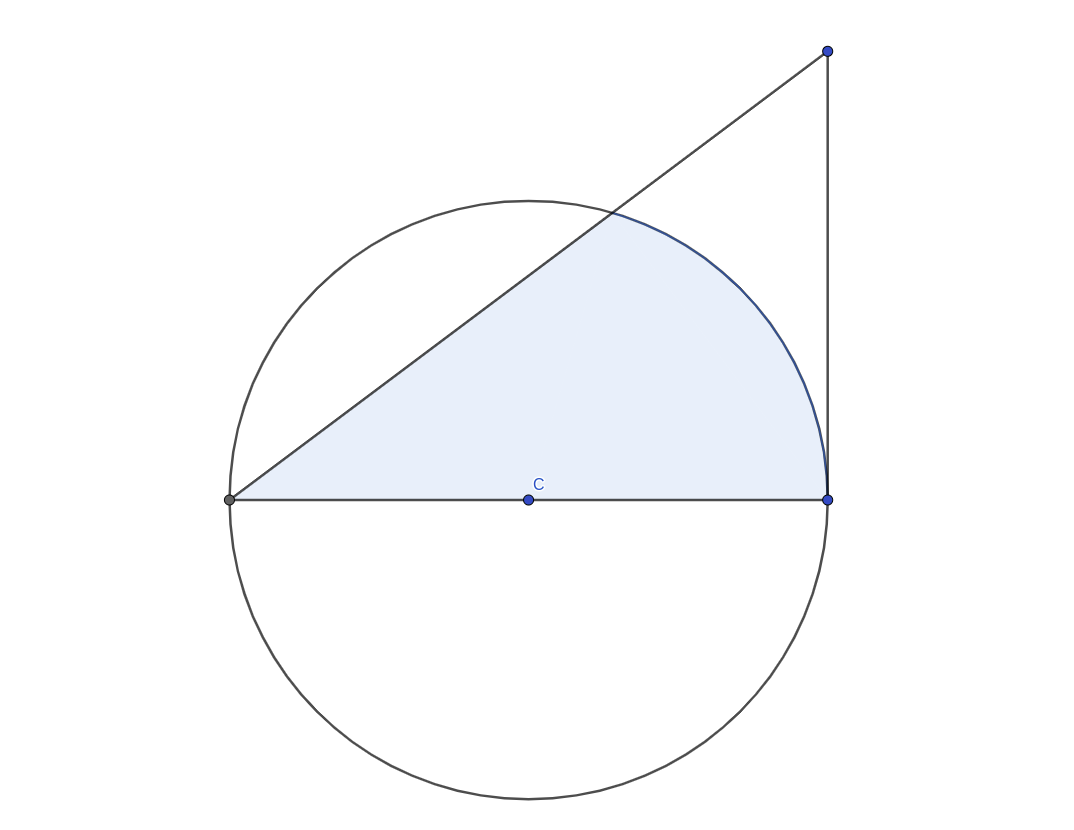
\includegraphics[scale=0.3]{\CWD/imagem.png}
\end{figure}

Ajude Felipe a resolver a questão.

%
% For input, use one of the following
%
\inputdesc{A entrada contém um único inteiro com o valor do raio $1 \leq R \leq 100$.}

%
% For output, use one of the following
%

\outputdesc{A saída deve ser a área de interseção das figuras. A saída será considerada correta se a diferença absoluta em relação à solução do juiz for no máximo $10^{-2}$.}

%\sampleio will look for files named sample-n.in and sample-n.sol (where n is 1, 2, 3...)
%in the documents directory and include them as samples.

\sampleio
